\section{Implementing the set computations}
\label{sec:implementing set computations}

In order to compute the sets $\tilde{E}_{k+j|k}$ and $\underline{V}_{k+j|k}$ which are needed by the RMPC formulation and are defined in the previous section, we need to use online reachability to compute the set in which $x_{k+j}$ lies in. To do this, we first define an online reachability based over-approximation scheme for the reach sets starting from the estimate at time $k$, $\hat{x}_k$.

 \subsection{Over-approximating the reach set of the nonlinear system}
\label{sec:x reach}

At time $k$, we need to compute the forward reach set, starting from $x_k$, for the next $N$ steps, for two purposes:
first, this is needed for defining the constraints on the input $v$ to the linearized dynamics.
Secondly, this is needed to compute a containing set for the estimation error in $z$-space.

In all but the simplest systems, forward reachable sets can not be computed exactly.
Moreover, the true state $x_k$ is not known.
Therefore we show how to compute an outer-approximation $\oaXset{k+j}{k},  j=0,\ldots, N$.
To do so we may use a reachability tool for nonlinear systems like RTreach??. 
A reachability tool computes an outer-approximation of the reachable set of a system starting from some set $\Xc \subset X$, subjet to inputs from a set $U$, for a duration $T \geq 0$. 
Denote this approximation by $\RT{\Xc}$.

At time $k$, the state estimate $\hx_{k}$ is known.
Therefore $x_k = \hx_{k} - e_k \in \hx_{k} \oplus (-E) \defeq \Xset{k}{k}$.
Propagating $\Xset{k}{k}$ forward one step through the continuous-time nonlinear dynamics yields $\Xset{k+1}{k}$, which is outer-approximated by $\RT{\Xset{k}{k}}$.
The estimate that the system will receive at time $k+1$ is therefore bound to be in the set $\RT{\Xset{k}{k}}  \oplus E$.
Since $0 \in E$, we maintain $\Xset{k+1}{k} \subset \RT{\Xset{k}{k}}  \oplus E$.
We define the outer-approximate reach set at $k+1$, computed at time $k$, to be 
\begin{equation*}
\label{eq:def Xk}
\oaXset{k+1}{k} \defeq  \RT{\Xset{k}{k}}  \oplus E \oplus  (-E)
\end{equation*}
%(The reason for adding the extra $-E$ term will be apparent in the proof to Thm.??).
Fig. \ref{fig:overreach_NL} shows a visualization of this approach.

More generally, for $1 \leq j \leq N$, we define the $j$-step reach set computed at time $k$ to be
\begin{eqnarray}
\label{eq:def Xkj}
\oaXset{k}{k} &\defeq&   \hx_{k} \oplus (-E) 
\nonumber
\\
\oaXset{k+j}{k} & \defeq& \RT{\oaXset{k+j-1}{k}} \oplus E \oplus (-E) 
\end{eqnarray}

The following holds by construction:
\begin{lemma}
	\label{lemma:xreach}
	For any time $k$ and step $j \geq 1$, the $j$-step reach set of the non-linear dynamics starting from $x_k$ is outer-approximated by $\oaXset{k+j}{k}$:
	$\Xset{k+j}{k} \subset \oaXset{k+j}{k}$.
\end{lemma}


\begin{figure*}
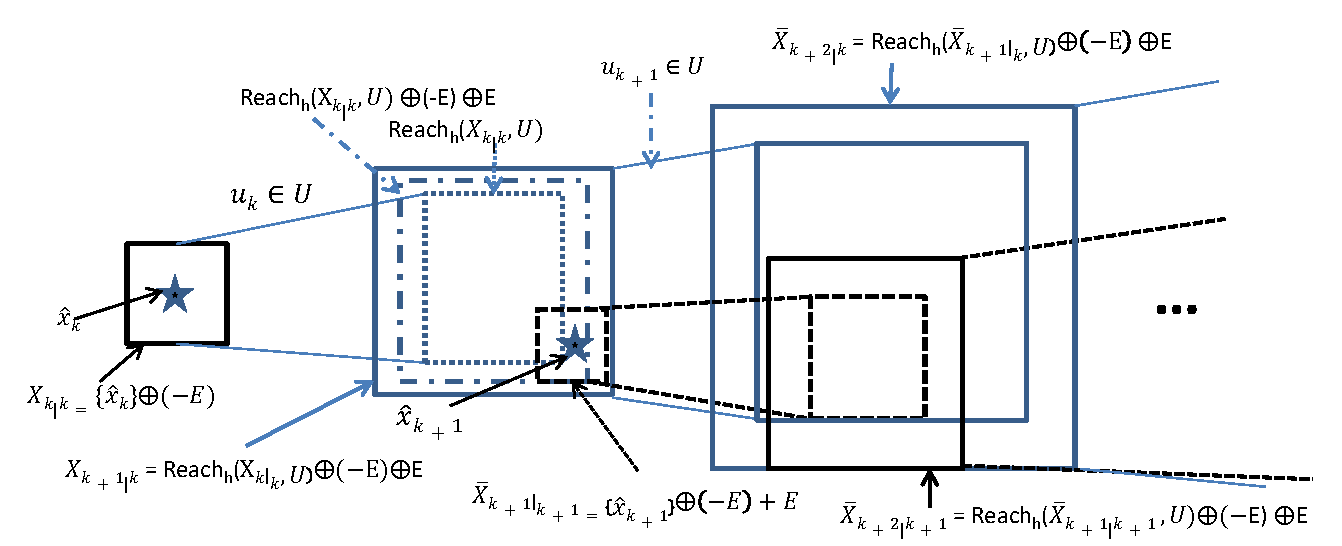
\includegraphics[scale=0.75]{figs/OverReachFigure_NL_scissored.pdf}
\caption{The over-approximated reachable sets for $x_{k+j}$, computed at time steps $k$, and correspondingly ay $k+1$ , used to compute $\tilde{E}_{k+j|k}$, $\underline{V}_{k+j|k}$. }
\label{fig:overreach_NL}
\end{figure*}

This construction of the outer-approximation permits us to prove recursive feasibility of the MPC controller,  because it causes the constraints of the MPC problem setup at time $k+1$ to be consistent with (stronger than) the constraints of the MPC problem setup at time $k$.
This was explicitly stated and proved in Thm. \ref{th:robust_feas}.

\subsection{Computing the inner approximation of the input set online}

Using the reachability over-approximations of Sec. \ref{sec:x reach} and the definition of the inner approximation of the input set for $v$ in Sec. \ref{}, we can compute $\underline{V}_{k+j|k}$ as:

\begin{subequations}
\begin{align}
\underline{V}_{k+j|k} &= \{v=[v_1,\ldots,v_{\dimV}]^T \such \nonumber \\
&\max_{x\in \oa{X}_{k+j|k}} \ua{v}_i(x)  \leq v_i \leq \min_{x \in \oa{X}_{k+j|k}} \oa{v}_i(x) \} 
\end{align}
\end{subequations}

Here, given the upper and lower bounds on $v$ can be computed using interval arithmetic by computing the rectangular bounds on $\oa{X}_{k+j|k}$ and $U$. 

Let us also define a global inner approximation that holds $\forall x \in X$ by 

\begin{subequations}
\begin{align}
\underline{V}_{inner-global} &= \{v=[v_1,\ldots,v_{\dimV}]^T \such \nonumber \\
&\max_{x\in X} \ua{v}_i(x)  \leq v_i \leq \min_{x \in X} \oa{v}_i(x) \} 
\end{align}
\end{subequations}


\subsection{Computing the bounding error set and disturbance approximations online}

In Sec. \ref{sec:approx dist}, since the set $X_{k+j|k}$ is unknown and we only have access to a state estimate at time $k$, we use the online reachable set over-approximation of Sec. \ref{sec:x reach} to obtain $\oa{X}_{k+j|k}$.
Then it holds that 
\[\min_{x \in \oa{X}_{k+j|k} e \in E}M_i(x)e \leq \te_{k+j}(i) \leq \max_{x \in \oa{X}_{k+j|k}, e \in E} M_i(x)e\]

To make these computations easier, in the examples we use one last over-approximation to simplify the optimizations needed to calculate the component-wise bounds, specifically, we use 
\begin{eqnarray}
\label{eq:Etilde}
\sum_{\ell=1}^{n} \min_{x \in \oa{X}_{k+j|k}, e \in E} M_{i\ell}(x)e(\ell)  \leq \te_{k+j}(i) 
\nonumber 
\\
\leq \sum_{\ell=1}^{n} \max_{x \in \oa{X}_{k+j|k}, e \in E} M_{i\ell}(x)e(\ell)
\end{eqnarray}
where $M_{i\ell}$ is the $(i,\ell)^{th}$ element of matrix $M$.
Therefore we define the rectangular error set $\tE_{k+j|k}$ to be the set of vectors $e = [e_1,\ldots, e_{\dimZ}]^T$ satisfying \eqref{eq:Etilde}. The max and min involved in this can be now either be analyticaly computed, or be computed quickly at run-time using interval arithmetic (by computing the rectangular bounds on $\oa{X}_{k+j|k}$. While this adds a level of conservation, it guarantees us that we obtain an upper bound on the max and a lower bound on the min, which allows us to proceed without violating any assumptions.

While the sets $\tE_{k}$ over-approximate the mapped estimation error, we also need to calculate containing sets for the process noise $\hat{w}$.
Recall that for all $k,j$, 
$\hz_{k+j+1} = z_{k+j+1} + \te_{k+j+1} = Az_{k+j}+Bv_k+w_{k+j} + \te_{k+j+1} =  A(\hz_{k+j} - \te_{k+j}) + Bv_k + w_{k+j} + \te_{k+j+1} = A\hz_{k+j} + Bv_k + w_{k+j} + \te_{k+j+1} - A \te_{k+j} = A\hz_{k+j} + Bv_k + \hw_{k+j+1}$.

Therefore 
\begin{equation}
\label{eq:What}
\hw_{k+j+1} \in \What_{k+j+1|k} \defeq W \oplus \tE_{k+j+1|k} \oplus(-A\tE_{k+j|k})
\end{equation}

We also define the set $\tilde{E}_{max}$, which is necessary for the terminal constraints of Eq. \ref{eq:P_f_def}. $\tilde{E}_{max}$ represents the worst case error bound on the estimation error $\tilde{e}_k$, and is computed similar to Eq. \ref{eq:Etilde}, but over the entire set $X$ and not reachable subsets of it:

\begin{eqnarray}
\label{eq:EtildeMax}
\sum_{\ell=1}^{n} \min_{x \in X, e \in E} M_{i\ell}(x)e(\ell)  \leq \te_{k}(i) 
\nonumber 
\\
\leq \sum_{\ell=1}^{n} \max_{x \in X, e \in E} M_{i\ell}(x)e(\ell)
\end{eqnarray}

$\What_{max}$ is then defined as:
\begin{equation}
\What_{max} = W \oplus \tilde{E}_{max} \oplus (-A\tilde{E}_{max})
\end{equation}


\subsection{Transforming between $x$-space and $z$-space}
\label{sec:transforming x to z}
Since we control the system in $z$-space, we need to compute a set $Z \subset \Re^\dimZ$ s.t. $z \in Z \implies x = \iT(z) \in X$, i.e. $Z \subset T(X)$.
Thus keeping the state $z$ of the linearized dynamics in $Z$ implies the nonlinear system's state $x$ remains in $X$.
Moreover, to check feasibility at time 0 of the MPC optimization, and for stability of the nonlinear dynamics, we need a subset $X_0 \subset X$ s.t. $x \in X_0 \implies z = T(x) \in Z$, i.e. $X_0 \subset \iT(Z)$.
Because $T$ can be an arbitrary diffeomorphism $Z$ and $X_0$ have to computed numerically.
\begin{itemize}
	\item Let $Z_1 \subset \Re^{\dimZ}$ be the rectangle with bounds in the $i^{th}$ dimension $[ \min_{x \in X} T_i(x),  \max_{x \in X} T_i(x) ]$, $i=1,\ldots, \dimX$.
	This over-approximates $T(X)$. 
	Next we need to prune it so it under-approximates $T(X)$. 
	\item Define $z_{in} \defeq \min \{ \|z \|_0 \such z \in Z_1, \iT(z) \notin X\}$.
	$z_{in}$ is the smallest-norm inadmissible $z$ in $Z_1$.
	Thus all points in the $\ell_0$-ball of radius $\|z_{in}\|$ are admissible, i.e. their pre-images via $\iT$ are in $X$.
	\item Let $R_z$ be the largest inscribed rectangle in the ball $B_z(0,\|z_{in}\|)$.
	Now we need to get the $x$-set that maps to $R_z$  (or a subset of it).
	\item Let $X_1 \subset X$ be the rectangle with bounds in the $i^{th}$ dimension $[\min_{z \in R_{z}} \iT_i(z),  \max_{z \in R_{z}} \iT_i(z) ]$.
	Again, this is an over-approximation of $\iT(R_{z})$, so it needs to be pruned.
	\item Define $x_{in} = \inf \{\|x\|_0 \such x \in X_1, T(x) \notin R_{z}\}$.
	Then every point in the $\ell_0$-ball $B_x(0, \|x_{in}\|) \subset X$ maps via $T$ to $R_{z}$
\end{itemize}
Therefore we choose $Z = R_z$ and $X_0$ to be the largest inscribed rectangle in $B_x(0,  \|x_{in}\|)$.

